\section{Search\_\-Target  Class Reference}
\label{classSearch__Target}\index{Search_Target@{Search\_\-Target}}
{\tt \#include $<$dil2al.hh$>$}

Inheritance diagram for Search\_\-Target::\begin{figure}[H]
\begin{center}
\leavevmode
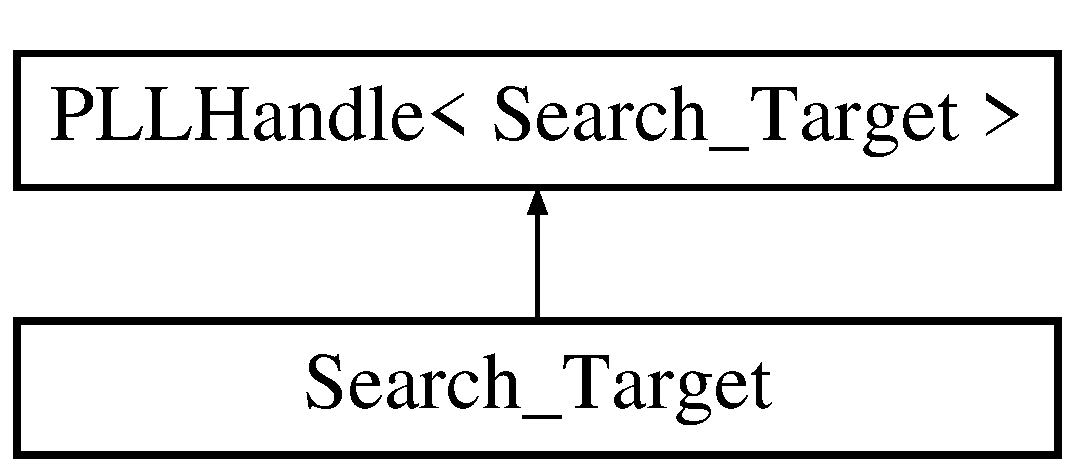
\includegraphics[height=2cm]{classSearch__Target}
\end{center}
\end{figure}
\subsection*{Public Methods}
\begin{CompactItemize}
\item 
{\bf Search\_\-Target} ({\bf PLLRoot}$<$ {\bf Search\_\-Result} $>$ $\ast$r, const char $\ast$s, const char $\ast$t, int f, bool l, {\bf Quick\_\-String\_\-Hash} $\ast$e=NULL)
\item 
{\bf Search\_\-Target} (const Search\_\-Target \&parent, const char $\ast$t)
\item 
{\bf String} {\bf Target} () const
\item 
long {\bf search} ()
\item 
long {\bf links} (const {\bf String} \&t)
\item 
void {\bf set\_\-searched} (int sval=1)
\item 
void {\bf reset\_\-searched} ()
\end{CompactItemize}
\subsection*{Protected Methods}
\begin{CompactItemize}
\item 
void {\bf check\_\-encountered} ()
\end{CompactItemize}
\subsection*{Protected Attributes}
\begin{CompactItemize}
\item 
{\bf PLLRoot}$<$ {\bf Search\_\-Result} $>$ $\ast$ {\bf results}
\item 
{\bf String} {\bf searchkey}
\item 
{\bf Target\_\-Access} {\bf target}
\item 
int {\bf followlinks}
\item 
bool {\bf localtargets}
\item 
{\bf Quick\_\-String\_\-Hash} $\ast$ {\bf encountered}
\item 
int {\bf searched}
\end{CompactItemize}


\subsection{Constructor \& Destructor Documentation}
\index{Search_Target@{Search\_\-Target}!Search_Target@{Search\_\-Target}}
\index{Search_Target@{Search\_\-Target}!Search_Target@{Search\_\-Target}}
\subsubsection{\setlength{\rightskip}{0pt plus 5cm}Search\_\-Target::Search\_\-Target ({\bf PLLRoot}$<$ {\bf Search\_\-Result} $>$ $\ast$ {\em r}, const char $\ast$ {\em s}, const char $\ast$ {\em t}, int {\em f}, bool {\em l}, {\bf Quick\_\-String\_\-Hash} $\ast$ {\em e} = NULL)\hspace{0.3cm}{\tt  [inline]}}\label{classSearch__Target_a0}




Definition at line 1037 of file dil2al.hh.

References check\_\-encountered(), followlinks, localtargets, and searched.

Referenced by links().



\footnotesize\begin{verbatim}1037 : results(r), searchkey(s), target(t), followlinks(f), localtargets(l), encountered(e), searched(0) { check_encountered(); }
\end{verbatim}\normalsize 
\index{Search_Target@{Search\_\-Target}!Search_Target@{Search\_\-Target}}
\index{Search_Target@{Search\_\-Target}!Search_Target@{Search\_\-Target}}
\subsubsection{\setlength{\rightskip}{0pt plus 5cm}Search\_\-Target::Search\_\-Target (const Search\_\-Target \& {\em parent}, const char $\ast$ {\em t})\hspace{0.3cm}{\tt  [inline]}}\label{classSearch__Target_a1}




Definition at line 1038 of file dil2al.hh.

References check\_\-encountered(), followlinks, localtargets, and searched.



\footnotesize\begin{verbatim}1038 : results(parent.results), searchkey(parent.searchkey), target(parent.target,t), followlinks(parent.followlinks-1), localtargets(parent.localtargets), encountered(parent.encountered), searched(0) { check_encountered(); } // relative to a parent target
\end{verbatim}\normalsize 


\subsection{Member Function Documentation}
\index{Search_Target@{Search\_\-Target}!check_encountered@{check\_\-encountered}}
\index{check_encountered@{check\_\-encountered}!Search_Target@{Search\_\-Target}}
\subsubsection{\setlength{\rightskip}{0pt plus 5cm}void Search\_\-Target::check\_\-encountered ()\hspace{0.3cm}{\tt  [protected]}}\label{classSearch__Target_b0}




Definition at line 278 of file search.cc.

References encountered, Quick\_\-String\_\-Hash::read(), searched, Target\_\-Access::TA\_\-FTP, Target\_\-Access::TA\_\-HTTP, Target\_\-Access::Target(), target, and Target\_\-Access::Type().

Referenced by Search\_\-Target().



\footnotesize\begin{verbatim}278                                       {
279         if (encountered) {
280                 if (encountered->read((const char *) target.Target())) searched = 1;
281                 else (*encountered) << (const char *) target.Target();
282         }
283         if ((!remotesearch) && ((target.Type()==Target_Access::TA_HTTP) || (target.Type()==Target_Access::TA_FTP))) searched = -1;
284 }
\end{verbatim}\normalsize 
\index{Search_Target@{Search\_\-Target}!links@{links}}
\index{links@{links}!Search_Target@{Search\_\-Target}}
\subsubsection{\setlength{\rightskip}{0pt plus 5cm}long Search\_\-Target::links (const {\bf String} \& {\em t})}\label{classSearch__Target_a4}




Definition at line 316 of file search.cc.

References String::contains(), String::empty(), generic\_\-remove\_\-name\_\-reference(), String::index(), PLLRoot$<$ Search\_\-Target $>$::link\_\-before(), PLLHandle$<$ Search\_\-Target $>$::Root(), String::SEARCH\_\-END, and Search\_\-Target().

Referenced by search().



\footnotesize\begin{verbatim}316                                           {
317         // Finds links in the text t and adds them to the list of targets
318         const BigRegex linksrx("[<][Aa][^>]+[Hh][Rr][Ee][Ff]");
319         const BigRegex lkendrx("[<][/][Aa][ \t]?[^>]*[>]");
320         const BigRegex urlstartrx("=[ \t]*\"?");
321         const BigRegex mailtorx("^[ \t]*[Mm][Aa][Ii][Ll][Tt][Oo][ \t]*:");
322         int i = 0;
323         while ((i=t.index(linksrx,String::SEARCH_END,i))>=0) {
324                 int urlstart = t.index(urlstartrx,String::SEARCH_END,i); // find URL start
325                 if (urlstart>=0) {
326                         int urlend;
327                         if (t[urlstart-1]=='"') urlend = t.index('"',urlstart); // find matching '"'
328                         else urlend = t.index(BRXwhite,urlstart); // find white-space terminated URL
329                         if (urlend>=0) {
330                                 String url(const_cast<String &>(t).at(urlstart,urlend-urlstart)); // get URL
331                                 generic_remove_name_reference(url);
332                                 if (!(url.empty() || url.contains(mailtorx))) {
333                                         // *** currently assumes breadth-first search
334                                         Search_Target * st = new Search_Target(*this,url);
335                                         Root()->link_before(st); // append st to list
336                                 }
337                         }
338                 }
339                 i = t.index(lkendrx,String::SEARCH_END,i); // find end of hyperlink
340         }       
341 }
\end{verbatim}\normalsize 
\index{Search_Target@{Search\_\-Target}!reset_searched@{reset\_\-searched}}
\index{reset_searched@{reset\_\-searched}!Search_Target@{Search\_\-Target}}
\subsubsection{\setlength{\rightskip}{0pt plus 5cm}void Search\_\-Target::reset\_\-searched ()\hspace{0.3cm}{\tt  [inline]}}\label{classSearch__Target_a6}




Definition at line 1045 of file dil2al.hh.

References searched.



\footnotesize\begin{verbatim}1045 { searched = 0; }
\end{verbatim}\normalsize 
\index{Search_Target@{Search\_\-Target}!search@{search}}
\index{search@{search}!Search_Target@{Search\_\-Target}}
\subsubsection{\setlength{\rightskip}{0pt plus 5cm}long Search\_\-Target::search ()}\label{classSearch__Target_a3}




Definition at line 287 of file search.cc.

References EOUT, followlinks, String::index(), PLLRoot$<$ Search\_\-Result $>$::link\_\-before(), links(), Target\_\-Access::read\_\-cleartext\_\-into\_\-String(), res, results, String::SEARCH\_\-END, searched, searchkey, Search\_\-Result::SR\_\-DIRECTORY\_\-ENTRY, Search\_\-Result::SR\_\-URL, PLLRoot$<$ Search\_\-Result $>$::tail(), Target\_\-Access::Target(), target, and Search\_\-Result::Type().



\footnotesize\begin{verbatim}287                            {
288         // Searches the target file for occurrences of searchkey and stores the results
289 #ifdef SEARCH_TARGET_DEBUG
290         EOUT << "dil2al: Search_Target::search(), followlinks=" << followlinks << ", target.Target() = " << target.Target() << '\n';
291 #endif
292         if (searched!=0) {
293                 if (verbose) {
294                         if (searched==1) EOUT << target.Target() << " already searched elsewhere\n";
295                         else EOUT << target.Target() << " restricted, do not search\n";
296                 }
297                 return 0;
298         }
299         String t;
300         if (!target.read_cleartext_into_String(t)) return -1;
301         int i = 0, res = 0; BigRegex skrx(searchkey);
302         while ((i=t.index(skrx,String::SEARCH_END,i))>=0) {
303                 Search_Result * r = new Search_Result(searchkey,target,t,skrx);
304                 if (((r->Type()==Search_Result::SR_DIRECTORY_ENTRY) || (r->Type()==Search_Result::SR_URL)) && (results->tail())) if (*(results->tail())==*r) {
305                         delete r; // try to avoid duplicates
306                         continue;
307                 }
308                 results->link_before(r);
309                 res++;
310         }
311         if (followlinks>0) links(t); // if followlinks>0 then links are sought and added to the search
312         searched = 1;
313         return res;
314 }
\end{verbatim}\normalsize 
\index{Search_Target@{Search\_\-Target}!set_searched@{set\_\-searched}}
\index{set_searched@{set\_\-searched}!Search_Target@{Search\_\-Target}}
\subsubsection{\setlength{\rightskip}{0pt plus 5cm}void Search\_\-Target::set\_\-searched (int {\em sval} = 1)\hspace{0.3cm}{\tt  [inline]}}\label{classSearch__Target_a5}




Definition at line 1044 of file dil2al.hh.

References searched.



\footnotesize\begin{verbatim}1044 { searched = sval; }
\end{verbatim}\normalsize 
\index{Search_Target@{Search\_\-Target}!Target@{Target}}
\index{Target@{Target}!Search_Target@{Search\_\-Target}}
\subsubsection{\setlength{\rightskip}{0pt plus 5cm}{\bf String} Search\_\-Target::Target () const\hspace{0.3cm}{\tt  [inline]}}\label{classSearch__Target_a2}




Definition at line 1041 of file dil2al.hh.

References Target\_\-Access::Target().



\footnotesize\begin{verbatim}1041 { return target.Target(); }
\end{verbatim}\normalsize 


\subsection{Member Data Documentation}
\index{Search_Target@{Search\_\-Target}!encountered@{encountered}}
\index{encountered@{encountered}!Search_Target@{Search\_\-Target}}
\subsubsection{\setlength{\rightskip}{0pt plus 5cm}{\bf Quick\_\-String\_\-Hash}$\ast$ Search\_\-Target::encountered\hspace{0.3cm}{\tt  [protected]}}\label{classSearch__Target_n5}




Definition at line 1027 of file dil2al.hh.

Referenced by check\_\-encountered().\index{Search_Target@{Search\_\-Target}!followlinks@{followlinks}}
\index{followlinks@{followlinks}!Search_Target@{Search\_\-Target}}
\subsubsection{\setlength{\rightskip}{0pt plus 5cm}int Search\_\-Target::followlinks\hspace{0.3cm}{\tt  [protected]}}\label{classSearch__Target_n3}




Definition at line 1025 of file dil2al.hh.

Referenced by search(), and Search\_\-Target().\index{Search_Target@{Search\_\-Target}!localtargets@{localtargets}}
\index{localtargets@{localtargets}!Search_Target@{Search\_\-Target}}
\subsubsection{\setlength{\rightskip}{0pt plus 5cm}bool Search\_\-Target::localtargets\hspace{0.3cm}{\tt  [protected]}}\label{classSearch__Target_n4}




Definition at line 1026 of file dil2al.hh.

Referenced by Search\_\-Target().\index{Search_Target@{Search\_\-Target}!results@{results}}
\index{results@{results}!Search_Target@{Search\_\-Target}}
\subsubsection{\setlength{\rightskip}{0pt plus 5cm}{\bf PLLRoot}$<${\bf Search\_\-Result}$>$$\ast$ Search\_\-Target::results\hspace{0.3cm}{\tt  [protected]}}\label{classSearch__Target_n0}




Definition at line 1022 of file dil2al.hh.

Referenced by search().\index{Search_Target@{Search\_\-Target}!searched@{searched}}
\index{searched@{searched}!Search_Target@{Search\_\-Target}}
\subsubsection{\setlength{\rightskip}{0pt plus 5cm}int Search\_\-Target::searched\hspace{0.3cm}{\tt  [protected]}}\label{classSearch__Target_n6}




Definition at line 1033 of file dil2al.hh.

Referenced by check\_\-encountered(), reset\_\-searched(), search(), Search\_\-Target(), and set\_\-searched().\index{Search_Target@{Search\_\-Target}!searchkey@{searchkey}}
\index{searchkey@{searchkey}!Search_Target@{Search\_\-Target}}
\subsubsection{\setlength{\rightskip}{0pt plus 5cm}{\bf String} Search\_\-Target::searchkey\hspace{0.3cm}{\tt  [protected]}}\label{classSearch__Target_n1}




Definition at line 1023 of file dil2al.hh.

Referenced by search().\index{Search_Target@{Search\_\-Target}!target@{target}}
\index{target@{target}!Search_Target@{Search\_\-Target}}
\subsubsection{\setlength{\rightskip}{0pt plus 5cm}{\bf Target\_\-Access} Search\_\-Target::target\hspace{0.3cm}{\tt  [protected]}}\label{classSearch__Target_n2}




Definition at line 1024 of file dil2al.hh.

Referenced by check\_\-encountered(), and search().

The documentation for this class was generated from the following files:\begin{CompactItemize}
\item 
{\bf dil2al.hh}\item 
{\bf search.cc}\end{CompactItemize}
